%  Created by Matthew Rásó-Barnett on 2009-08-10	
\documentclass[11pt,a4paper,oneside]{article}

% Setup for fullpage use - Reduces the margins at the sides
\usepackage{fullpage}

% -------------------------------------

% More symbols
\usepackage{amssymb}
\usepackage{amsmath}
\usepackage{latexsym}

\usepackage[parfill]{parskip}  % Activate to begin paragraphs with an empty line
\usepackage{epstopdf}
\usepackage{mathrsfs} % mathrsfs is for producing the curly H for Hilbert space
\DeclareMathAlphabet{\mathpzc}{OT1}{pzc}{m}{it} % This is to define another curly type of font called with \mathpzc{ }
\usepackage{dsfont} % For identity symbol

\usepackage[pdftex]{graphicx}
\usepackage[usenames,dvipsnames]{color}

% -------------------------------------

% For Source code, use the listings environment
\usepackage{listings}
\usepackage{courier}
\lstset{
	language=C,
	basicstyle=\scriptsize\ttfamily, 
	numberstyle=\tiny,          
	numbersep=5pt,              
	tabsize=2,                  
	extendedchars=true,         
	breaklines=true,            
	keywordstyle=\color{red},
	stringstyle=\color{white}\ttfamily, 
	showspaces=false,           
	showtabs=false,             
	xleftmargin=17pt,
	framexleftmargin=17pt,
	framexrightmargin=5pt,
	framexbottommargin=4pt,
	%backgroundcolor=\color{lightgray},
	showstringspaces=false,          
	keywordstyle=\color{blue},
	commentstyle=\color{OliveGreen},
	stringstyle=\color{red},
	numbers=left,
	numberstyle=\tiny,
	numbersep=5pt,
	breaklines=true,
	emph={label}
}
\lstloadlanguages{% Check Dokumentation for further languages ...
	%C
	C++
	%XML
	%HTML
	%Java
}
%\DeclareCaptionFont{blue}{\color{blue}} 
%\captionsetup[lstlisting]{singlelinecheck=false, labelfont={blue}, textfont={blue}}
\usepackage{caption}
\DeclareCaptionFont{white}{\color{white}}
\DeclareCaptionFormat{listing}{\colorbox[cmyk]{0.43, 0.35, 0.35,0.01}{\parbox{\textwidth}{\hspace{15pt}#1#2#3}}}
\captionsetup[lstlisting]{format=listing,labelfont=white,textfont=white, singlelinecheck=false, margin=0pt, font={bf,scriptsize}}

% -------------------------------------

% For Floats
\usepackage{float}

% New float for source code examples
\floatstyle{plain} 
\newfloat{sourcecode}{!htb}{}{}
\floatname{sourcecode} 

% Multipart figures
\usepackage{subfig}

% -------------------------------------


\title{UCNSIM Design Overview}
\author{Matthew Raso-Barnett}

\date{10-08-2009}

\begin{document}

\DeclareGraphicsExtensions{.pdf, .jpg, .png}


\maketitle


%=-=-=-=-=-=-=-=-=--=-=-=-=-=-=-=-=-=-=-=-=-=-=-=-=-=-=-=-=-=-=-=-=-=-=-
% Begin Document
%=-=-=-=-=-=-=-=-=--=-=-=-=-=-=-=-=-=-=-=-=-=-=-=-=-=-=-=-=-=-=-=-=-=-=-
\section{Introduction}

This document intends to give a brief introduction to some of the key elements we have faced in the process of creating a UCN-tracking program with ROOT. It is by no means meant to be a comprehensive overview of the entire program, as that would be a far larger document. Instead we have chosen to focus on giving a small flavour of the how the basic calculation to find the intersection of a parabolic-trajectory with a surface boundary is carried out, and the impact/challenges of trying to adapt ROOT to incorporate this calculation. Hopefully by reading this document, the reader will have an idea of how the calculation is carried out, and an understanding of the two major C++/ROOT specific 
problems and how they have forced the design of the program into difficult territory. Finally this document is a work in progress and will be added to overtime to add more and more detail as and when we find the time, eventually forming a more complete overview of the program.

\section{Tracking Particles Under Gravity Through Parabolic Ray-Tracing}

There are two essential features one must consider when developing a simulation of ultra-cold neutrons (UCN) moving through a guide-tube: how you intend to simulate a particle's motion under gravity and how you intend to implement the physics of ultra-cold neutrons reflecting from a boundary. The physics of UCN reflecting from a boundary is where one will employ monte-carlo techniques to reproduce the observed behaviour of UCN in experiments, such as using quantum mechanics to calculate the probability of a UCN being absorbed/reflected at every bounce to build up the expected number density at the end of the guide-tube. 

The physics of UCN moving under gravity is far more straight forward. We all know the basic equations of motion of a particle moving under the earth's gravitational field,

\begin{equation}
X_{i}(t) = X_{i}(0) + \dot{X}_{i}(0)t + \frac{1}{2}g\hat{G}_{i}t^{2} \ \ \ \ \ \ \ \ \ \ \mbox{where,} \ i = 1, 2, 3
\label{eqn:GravitationalMotion}
\end{equation}

where, $X_{i}(t)$ is the position vector of the particle at a time $t$, $g$ is the gravitational free-fall acceleration of a particle and where $\hat{G}_{i}$ is a unit vector signifying the direction of the earth's gravitational field - usually pointing straight down along the z-axis by convention. 

When it comes to building a simulation, the problem of tracking UCN under gravity is a much harder challenge. Just propagating a point or ray through a volume, along a straight line, is a rather involved problem that has, fortunately,  been worked out many times in the past and is now built into ROOT itself - with native methods designed to calculate the distance between a particle's current point in a geometry and the next boundary that point will intersect as it travels along its current direction. The difficulty here is in determining exactly (and correctly!), at every step of the way, where in a geometry hierarchy (such as a series of nested boxes - think of Matroska dolls!) our particle actually is. There are many pitfalls to be found when propagating to, and ensuring that one crosses, a boundary, so when we wish to build a simulation that also introduces the possibility of reflection from a boundary, we have to be extremely careful with issues such as this. 

\subsection{A Typical Calculation: The Plane}

To begin with we will run through the basic calculations involved in performing a single ray-tracing-like `step' of a particle under gravity. 

Consider a particle with a position vector $X_{i}(t_{0}) = (x(t_{0}), y(t_{0}), z(t_{0}))$ that is within a coordinate system that is defined by some master volume that we typically refer to as the world or global frame. Now consider the same particle that is now enclosed within another volume that is rotated with respect to the global frame, figure~\ref{fig:NestedBox}

\begin{figure}[!htbp] 	
\begin{center}
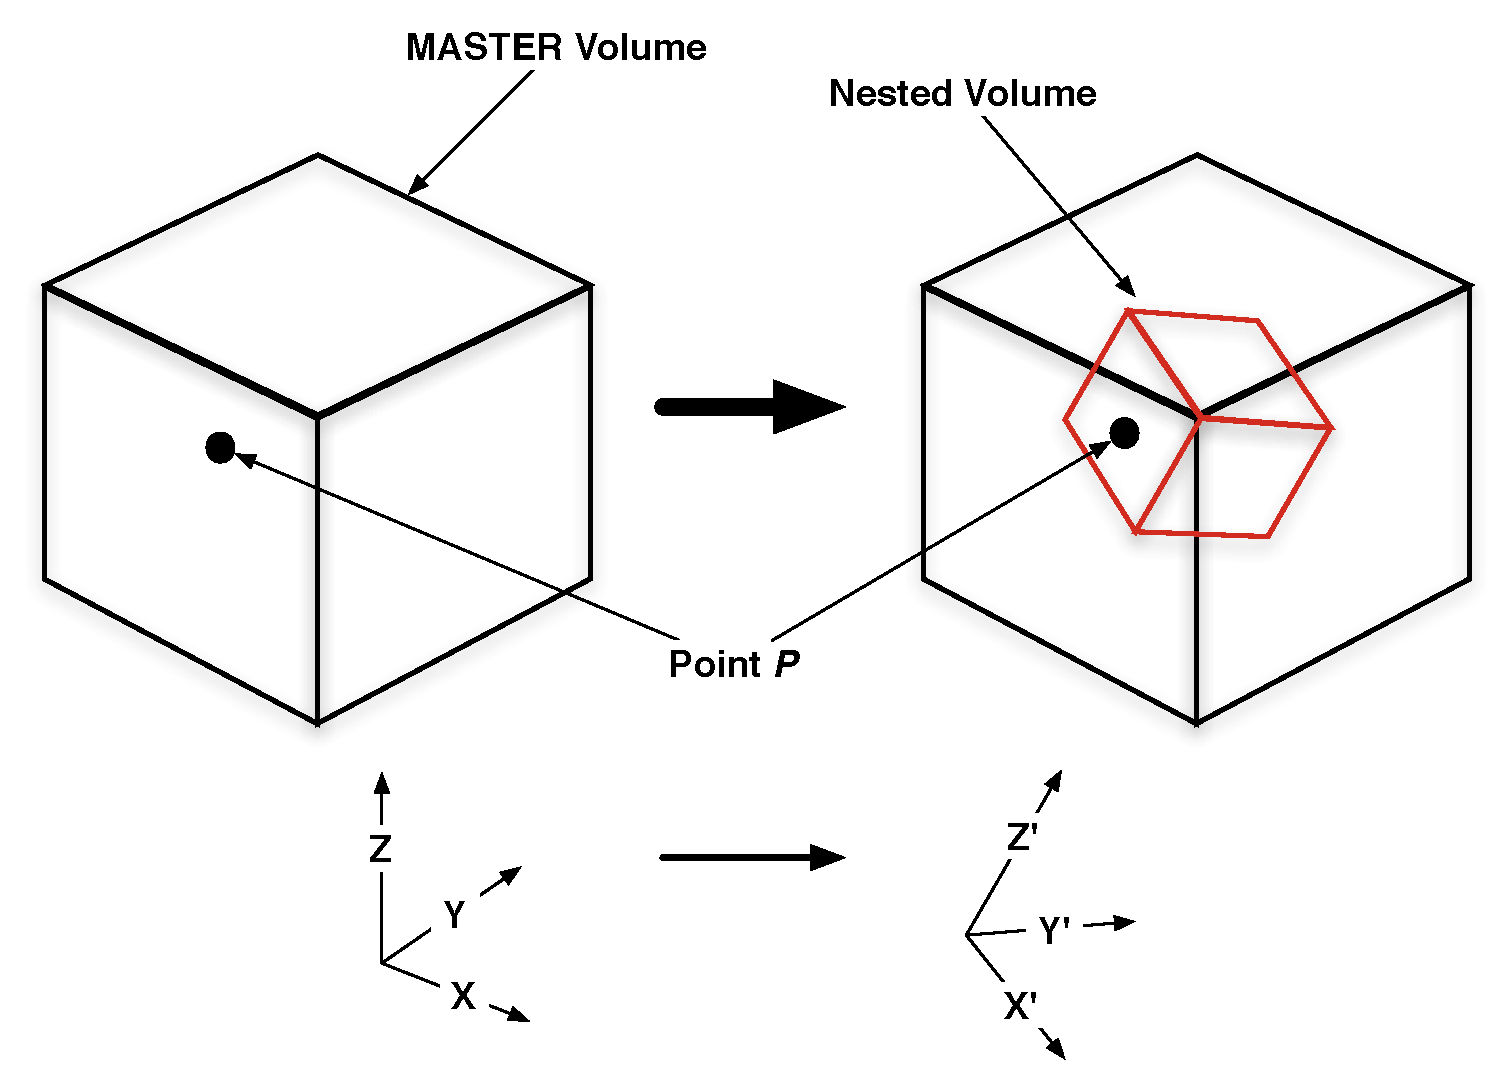
\includegraphics[scale=0.4]{designdocumentimages/fig1-NestedBox}
\end{center}
\caption{A simple geometry hierarchy of a single box, rotated with respect to the global volume.}
\label{fig:NestedBox}
\end{figure}

where the particle at point $P$, transformed into the `local' coordinate frame of the rotated box, is given by $X^{\prime}_{i}(t_{0}) = (x^{\prime}(t_{0}), y^{\prime}(t_{0}), z^{\prime}(t_{0})) = M_{ij}X_{j}$, and where $M_{ij}$ is some transformation matrix representing the rotation of the box. 

Whenever we perform a calculation we will always work in the local coordinate frame of the volume which the point is contained by. Then once we have found the intersection point of the next boundary in the local frame, we transform our point back to the global coordinate system and do the actual propagation there. 

\subsubsection*{Calculate Intersection With Boundary}

Our particle has an initial momentum of course, $P_{i}(t_{0})$, which in the local frame is given as above by $P^{\prime}_{i}(t_{0})$. It is clear that, as long as the particle has a non-zero momentum that there will always be exactly two intersections with the boundaries of the box (ie: an entry point and an exit point), as depicted in figure~\ref{fig:IntersectionWithBox}.

\begin{figure}[!htbp] 
\begin{center}
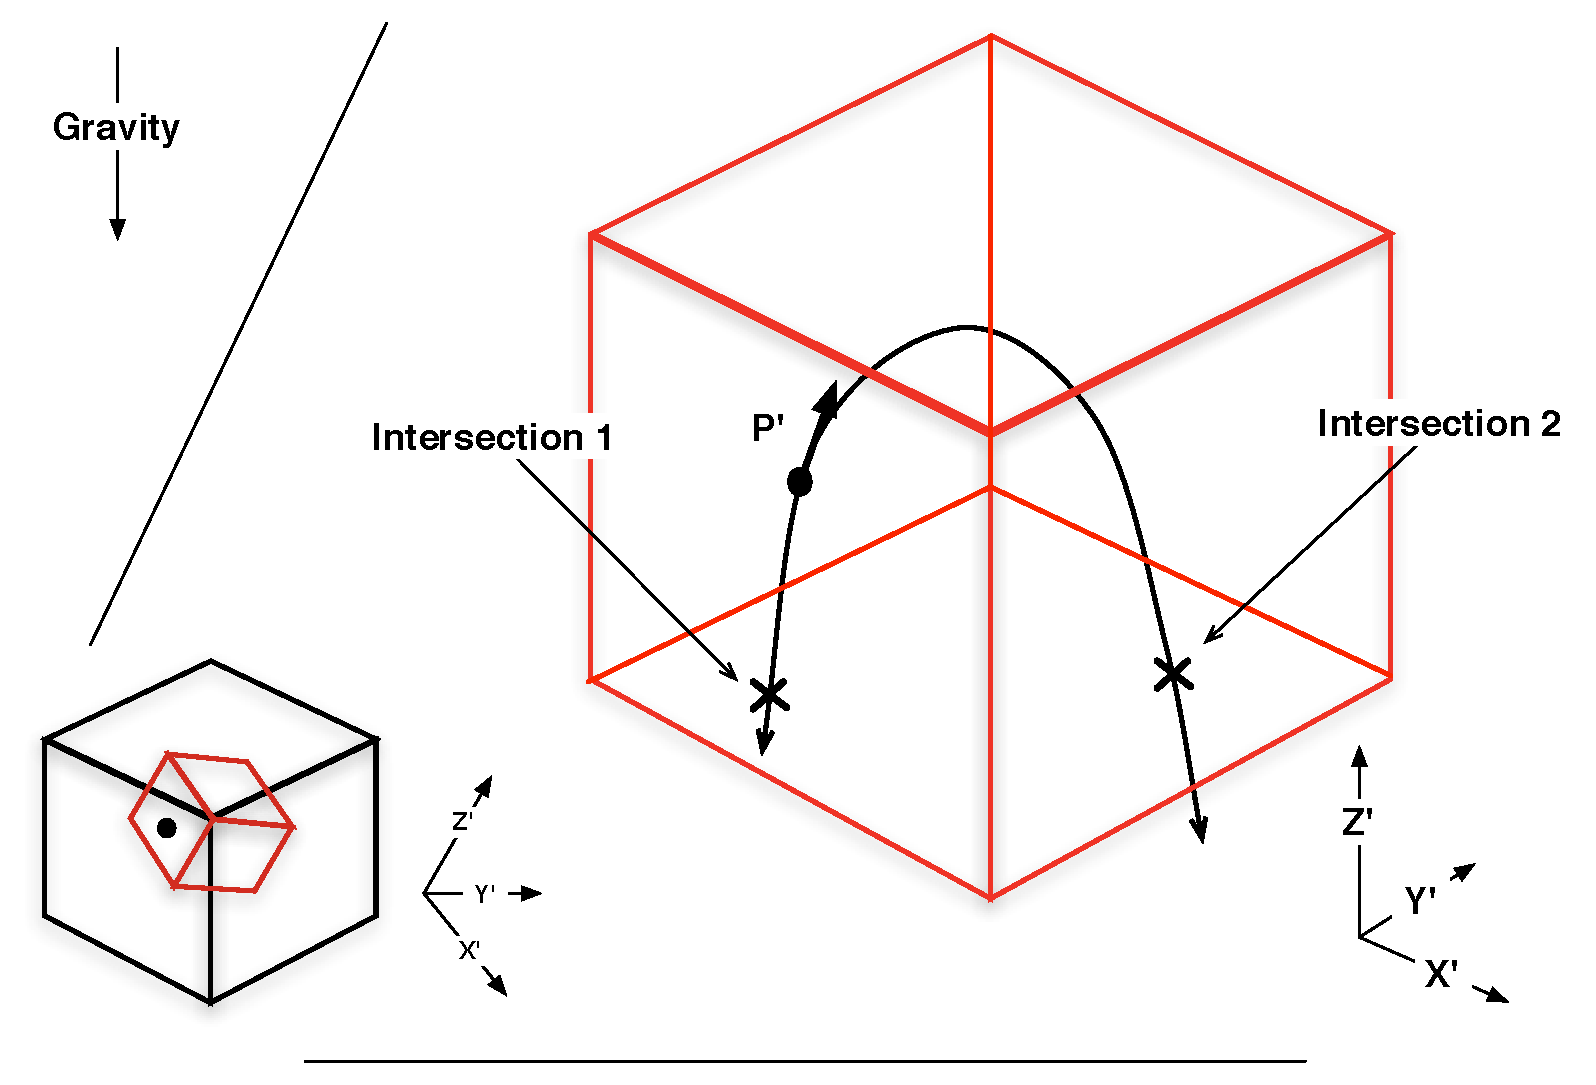
\includegraphics[scale=0.4]{designdocumentimages/fig2-IntersectionWithBox}
\end{center}
\caption{An example of a single track inside the box, viewed from the local coordinate frame of the box. There will always be at least two intersections with the boundaries of the box}
\label{fig:IntersectionWithBox}
\end{figure}

The aim of a parabolic tracking routine is to calculate these intersection points. To do this, we must consider each boundary in turn, so for the box that means we consider each side of the box as a separate plane, and determine if and where there is an intersection. So for example, consider that we are working in the local coordinate frame of the box, and we have a single non-zero component of the momentum, say $p^{\prime}_{x}(t_{0}) \neq 0$, and a single corresponding boundary of the box, for example, the positive-X boundary $x^{\prime}(t) = +L, -\infty < y^{\prime}(t) < +\infty, -\infty < z^{\prime}(t) < +\infty$.

Using equation~\ref{eqn:GravitationalMotion} we can solve the x-component equation to find the time of intersection with the $x^{\prime}(t) = +L$ plane. 

\begin{eqnarray}
x^{\prime}(t) = +L &=& x(0) + \dot{x}^{\prime}(0)t + \frac{1}{2}g\hat{G}_{x^{\prime}}t^{2} \\
\Rightarrow \ \ \	 0 &=& (x^{\prime}(0) - L) + \dot{x}^{\prime}(0)t + \frac{1}{2}g\hat{G}_{x^{\prime}}t^{2} \\
\Rightarrow \ \ \	 0 &=& at^{2} + bt + c
\label{eqn:SolveForBoundaryIntersection}
\end{eqnarray}

which is a quadratic equation for $t$. This equation gives all possible intersections with the entire $x^{\prime}(t) = +L$ plane as depicted in figure~\ref{fig:IntersectionWithPlane}; two solutions represent a particle that crosses the boundary twice, one solution means one intersection and so on. A negative solution means the parabola intersects the boundary but only in the past when $t$ is extended back to $-\infty$.

\begin{figure}[!htbp] 
\begin{center}
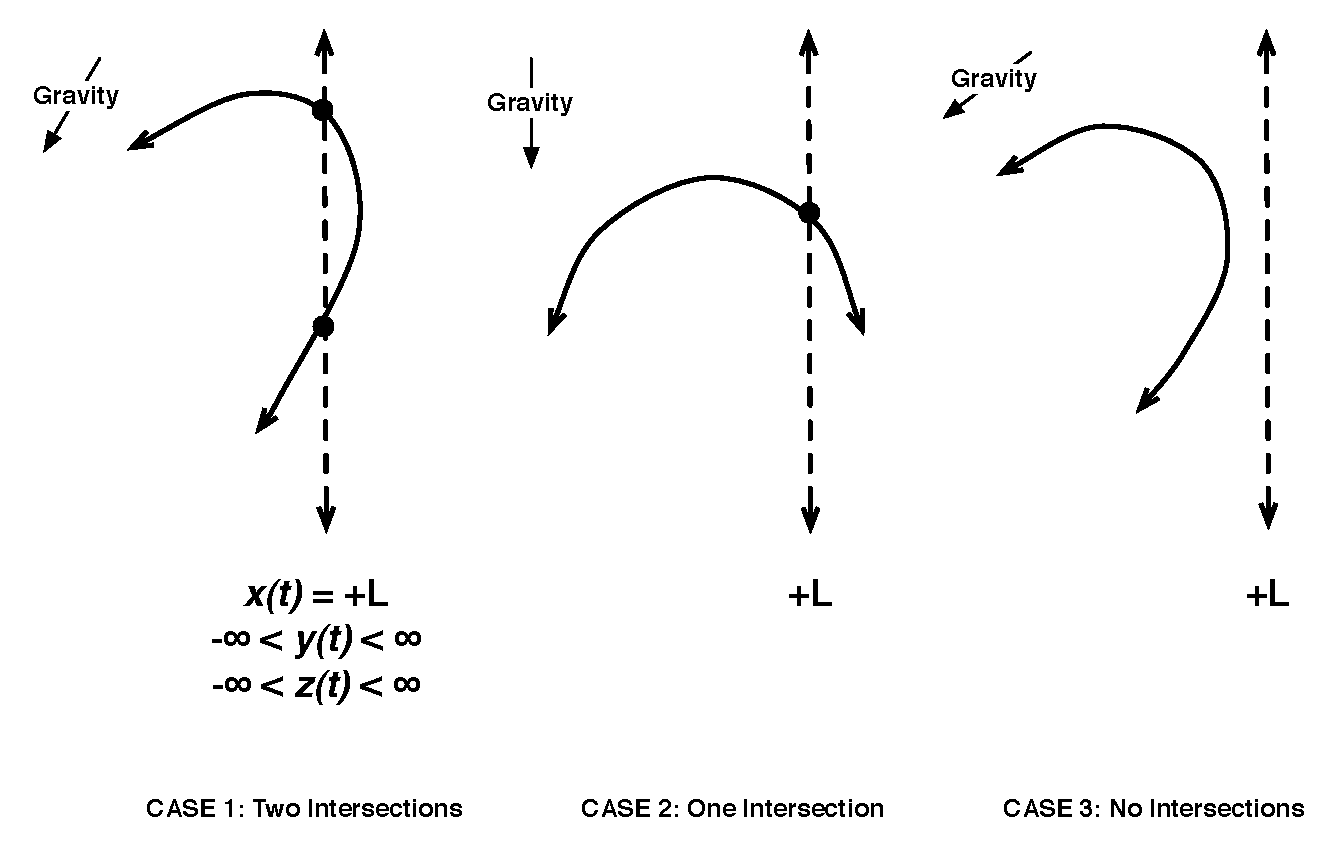
\includegraphics[scale=0.6]{designdocumentimages/fig3-IntersectionWithPlane}
\end{center}
\caption{An example of a one-dimensional parabola crossing a single plane/line.}
\label{fig:IntersectionWithPlane}
\end{figure}

So if our particle starts inside the box, and therefore must intersect one of the boundaries along its trajectory, we must solve the equation shown above for each of the six boundaries of the box $\pm X, \pm Y, \pm Z$ and then find the \textbf{smallest}, \textbf{positive}, \textbf{non-zero} value of $t$ from the possible solutions, which represents the intersection point with the boundary.

  
\subsubsection*{Calculate Distance Travelled Along Parabola}

Now that we have found the time, $t_{1}$, of intersection of the particle's trajectory with the nearest boundary, we can safely make a `step' and move our particle to this point. We then need to calculate the distance travelled in this step which can be accomplished as follows:

Consider an element of path length,
\begin{equation}
ds = \sqrt{dx^{2} + dy^{2} + dz^{2}}
\end{equation}

Hence, the arc length of a curve is given by,
\begin{equation}
L = \int_{curve} ds
\end{equation}

Substituting and rearranging, 
\begin{eqnarray}
\Rightarrow \ \ \ \ L &=& \int_{t_{0}}^{t_{1}} dt \sqrt{ \left( \frac{dx}{dt} \right)^{2} + \left( \frac{dy}{dt} \right)^{2} + \left( \frac{dz}{dt} \right)^{2} } \\
\Rightarrow \ \ \ \ \ &=& \int_{t_{0}}^{t_{1}} dt \sqrt{ \left( v_{x}(0) + g\hat{G}_{x}t \right)^{2} + \left( v_{y}(0) + g\hat{G}_{y}t \right)^{2} + \left( v_{z}(0) + g\hat{G}_{z}t \right)^{2} } \\
\Rightarrow \ \ \ \ \ &=& \int_{t_{0}}^{t_{1}} dt \sqrt{ |v(0)|^{2} + 2g\left( v_{x}(0)\hat{G}_{x} + v_{y}(0)\hat{G}_{y} + v_{z}(0)\hat{G}_{z} \right)t + g^{2}t^{2} }
\end{eqnarray}

Which is of the form, 
\begin{equation}
L = \int dt \sqrt{ at^{2} + bt + c}
\end{equation}

and can be solved by parts or looked up in integral tables,
\begin{equation}
L = \frac{(2at + b)\sqrt{at^{2} + bt + c}}{4a} + \frac{(4ac - b^{2})}{8a\sqrt{a}}\arcsin \left[ \frac{2at + b}{\sqrt{4ac - b^{2}}} \right]
\label{eqn:ArcLength}
\end{equation}

\subsubsection*{Time to Boundary From Outside and Other Shapes}

So above we have seen a simple calculation to find the time of intersection for a parabola and a plane, and the general result for the distance along a parabola. With these two formulae, we could put together a basic simulation for a particle in a box, by calculating the time to intersect a boundary for each of the six boundaries of the box, and taking the smallest, positive, non-zero value. 

However if our particle starts from outside the box, we have an extra step to perform. This is to check that the smallest, positive, non-zero value for the time to intersect, actually corresponds to a point on the box, as demonstrated in figure~\ref{fig:TimeFromOutside}

\begin{figure}[!htbp] 
\begin{center}
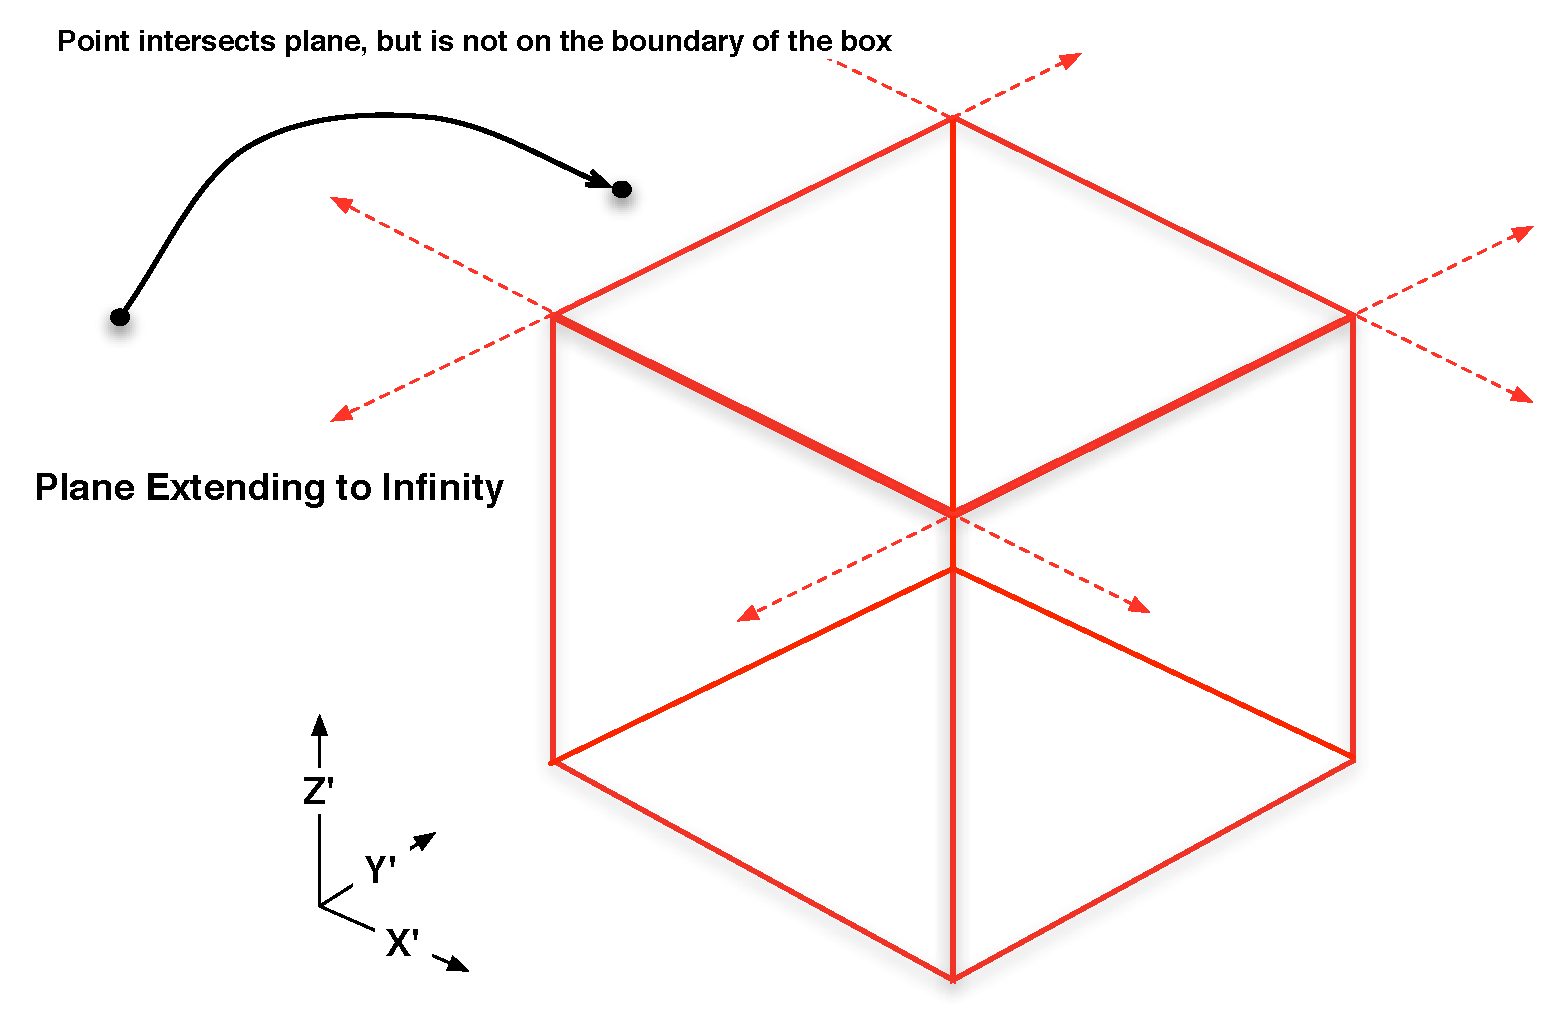
\includegraphics[scale=0.4]{designdocumentimages/fig4-TimeFromOutside}
\end{center}
\caption{Approaching the volume from outside.}
\label{fig:TimeFromOutside}
\end{figure}

All of the above discussion applies to other shapes such as the cylinder or the torus. The only difference with these shapes is in solving the equations to find the intersections with more complicated surfaces. These equations are also of higher order - recall that the plane requires us to solve a quadratic, order-2 polynomial; the cylinder requires a quartic, order-4 polynomial, and the torus requires an order-8 polynomial (that cannot be solved analytically). 

To show this explicitly in the case of the cylinder, consider a cylinder aligned with its horizontal dimension along the z-axis, and the circular boundary in the X-Y plane. The two ends of the tube at $z = \pm L$ can be solved for just as before, considering them as two infinite planes. The circular boundary however requires us to solve a much harder equation. The equation of a circle of radius $R$ in the X-Y plane is, $R^{2} = x^{2} + y^{2}$. Substituting in the equations of motion of our particle under gravity gives, 
\begin{eqnarray}
0 &=& \Big(\frac{1}{2}g\hat{G}_{x}t^{2} + v_{x}(0)t + x(0)\Big)^{2} + \Big(\frac{1}{2}g\hat{G}_{y}t^{2} + v_{y}(0)t + y(0)\Big)^{2} - R^{2} \\
\Rightarrow &=& t^{4}\Big(\frac{1}{2}g^{2} \left[ \hat{G}_{x}^{2} + \hat{G}_{y}^{2} \right]\Big) + t^{3}\Big(g\left[ \hat{G}_{x} v_{x}(0) + \hat{G}_{y} v_{y}(0) \right]\Big) + t^{2} \Big( g \left[ \hat{G}_{x}x(0) + \hat{G}_{y}y(0) \right] \\ 
&+& \left[ v_{x}^{2}(0) + v_{y}^{2}(0) \right]\Big) + t\Big(2 \left[ v_{x}(0)x(0) + v_{y}(0)y(0) \right]\Big) + (x^{2}(0) + y^{2}(0) - R^{2}) \\
\Rightarrow &=& at^{4} + bt^{3} + ct^{2} + dt + e
\end{eqnarray}

which is the standard form of a quartic polynomial. This of course simply reflects the fact that there can be at most four possible intersections of a parabola and a circle, whereas there can be at most eight possible intersections between the torus and the parabola, hence the order-8 polynomial. So after solving the polynomial equation for $t$, we can again go through the process of finding the smallest, non-zero, positive value that corresponds to a point on the boundary. 

\section{Designing a Particle Tracking Routine with ROOT}

\subsection{Overview of the Stepping Algorithm}

With the central calculation outlined in the previous section, the next task is to implement these methods into a larger `Find the next boundary and step to that point' algorithm. Having covered the basics of the type of calculation that we do, leaving aside the specific algorithm used to solve the polynomials, we outline a typical step when a track propagates in figure~\ref{fig:PropagationLoop}. 

\begin{figure}[!htbp] 
\begin{center}
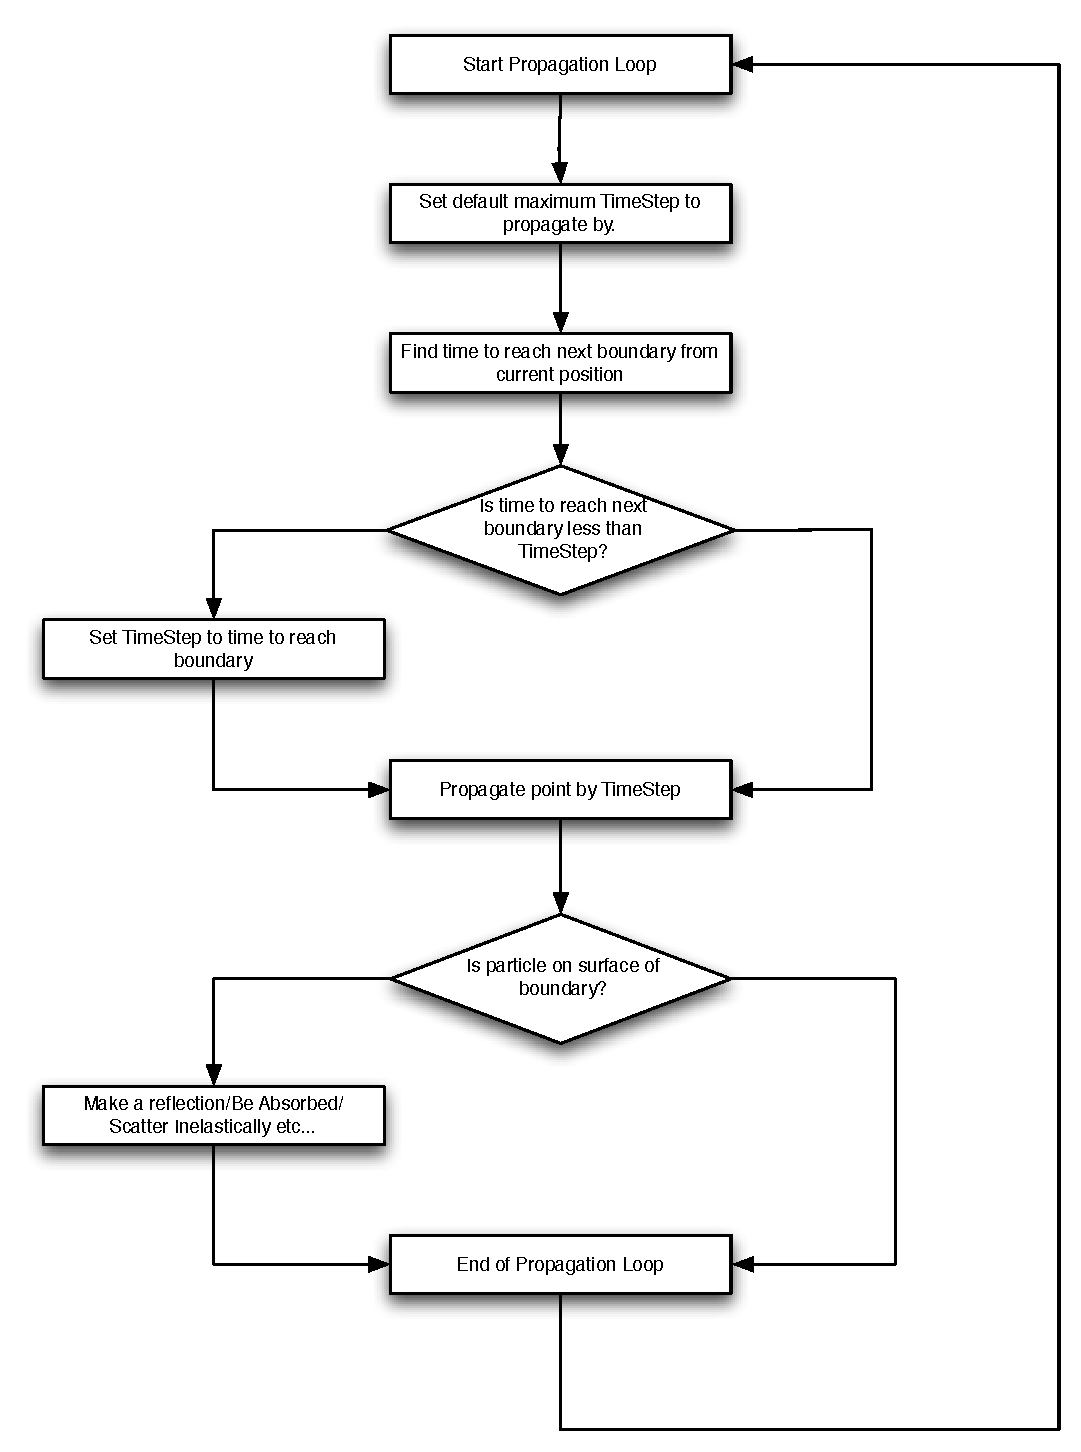
\includegraphics[scale=0.6]{designdocumentimages/fig5-PropagationLoop}
\end{center}
\caption{The basic decisions involved in a typical propagation loop}
\label{fig:PropagationLoop}
\end{figure}

\subsection{ROOT Navigation and Geometry}

One of the major obstacles when implementing an algorithm of this sort is taking care of where your point is located within the geometry. To tackle this, UCNSIM uses ROOT as a basis for its geometries and navigation through the various volumes in the geometry. Below, figure~\ref{fig:RootGeometries}, illustrates some examples of the types of volumes that can be built with ROOT. 

\begin{figure}[!htbp] 
\centering 
\subfloat[A tube]{\label{fig:Tube}
\includegraphics[width=0.3\textwidth]{designdocumentimages/cuttube.png}} \hspace{2mm} 
\subfloat[A torus]{\label{fig:Torus}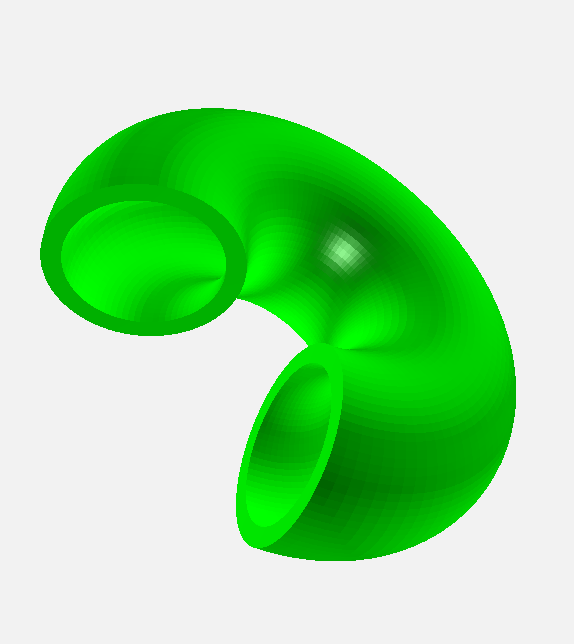
\includegraphics[width=0.3\textwidth]{designdocumentimages/torus.png}} \hspace{2mm}
\subfloat[Atlas Detector]{\label{fig:Atlas}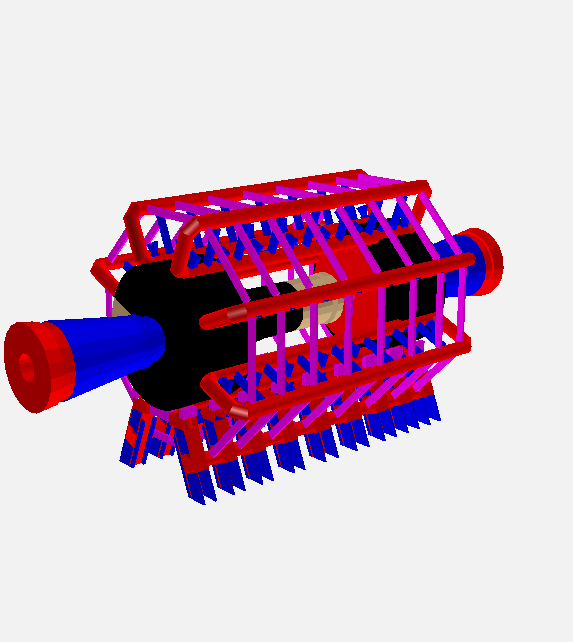
\includegraphics[width=0.3\textwidth]{designdocumentimages/atlas.png}} \hspace{2mm}
\caption{Some examples of ROOT geometries} 
\label{fig:RootGeometries} 
\end{figure}

ROOT geometries are built and maintained by the ROOT package TGEO. This package contains classes for building volumes (TGeoVolume, TGeoShape, TGeoBuilder), assigning volumes a specific material/medium (TGeoMaterial, TGeoMedium), creating tracks (TGeoTrack, TParticle) and providing navigation features for these tracks (TGeoNavigator) so that straight away, we have the tools to perform basic particle tracking along straight lines, such as that used for ray-tracing. At the head of all these classes is the geometry manager (TGeoManager), which stores lists of all the volumes, materials, tracks, orientations and is the means through which the user/program can query the geometry for information on its current status. 

The core of a ROOT geometry are of course the TGeoVolume objects. Volumes are made from a TGeoShape object, such as a Box (TGeoBBox) or tube (TGeoTube), and a medium (TGeoMedium). Volumes can contain other volumes however, and if one pictures a complex geometry, such as the Atlas geometry pictured above, figure~\ref{fig:Atlas}, there are many volumes that contain other smaller volumes inside, which themselves contain smaller volumes, working all the way down until you reach the smallest components of the experiment. For systems such as ROOT, these structures of nested volumes are stored in a logical \textbf{hierarchy}, where each volume is contained by a single `parent' volume, which may or may not be contained by larger parent, and so on, until you reach the TOP, or master volume.

A single volume object does not know its position in this hierarch however. The volume only knows the information about placement of all the other volumes that it contains, its `daughter' volumes. The crucial link tying the whole hierarchy of volumes together are the TGeoNode objects. A node is essentially a positioned volume, holding a single volume and a transformation object (TGeoMatrix) specifying the position/orientation of that volume inside its parent volume. Therefore every volume contains a list of TGeoNode objects specifying which daughter volumes it contains and where it is positioned relative to itself. 

In order to provide navigation features a volume needs to be able to find the proper container of the current point of a track, which could be the volume itself, one of its daughter volumes or none if the point is actually outside the volume. Volumes also need to provide navigation methods such as computing the distance from the current point to the next boundary or which daughter volume will be crossed first. These navigational features are implemented at the shape level, and the local mother-daughter relationship is handled at the Volume level. 

Shapes in ROOT are the main example of polymorphism in the TGEO package, which is an important distinction when looking at the design of UCNSIM in the next section. The class TGeoShape defines the basic shape interface which is implemented by all the specific shapes that inherit from it, as shown in figure~\ref{fig:ShapeInheritance}. Pointers to shape objects in ROOT are almost always passed as the base type TGeoShape, and rely on polymorphism to provide the correct shape-dependent implementation of the function call based on the real underlying type of the object. 

\begin{figure}[!htbp] 
\begin{center}
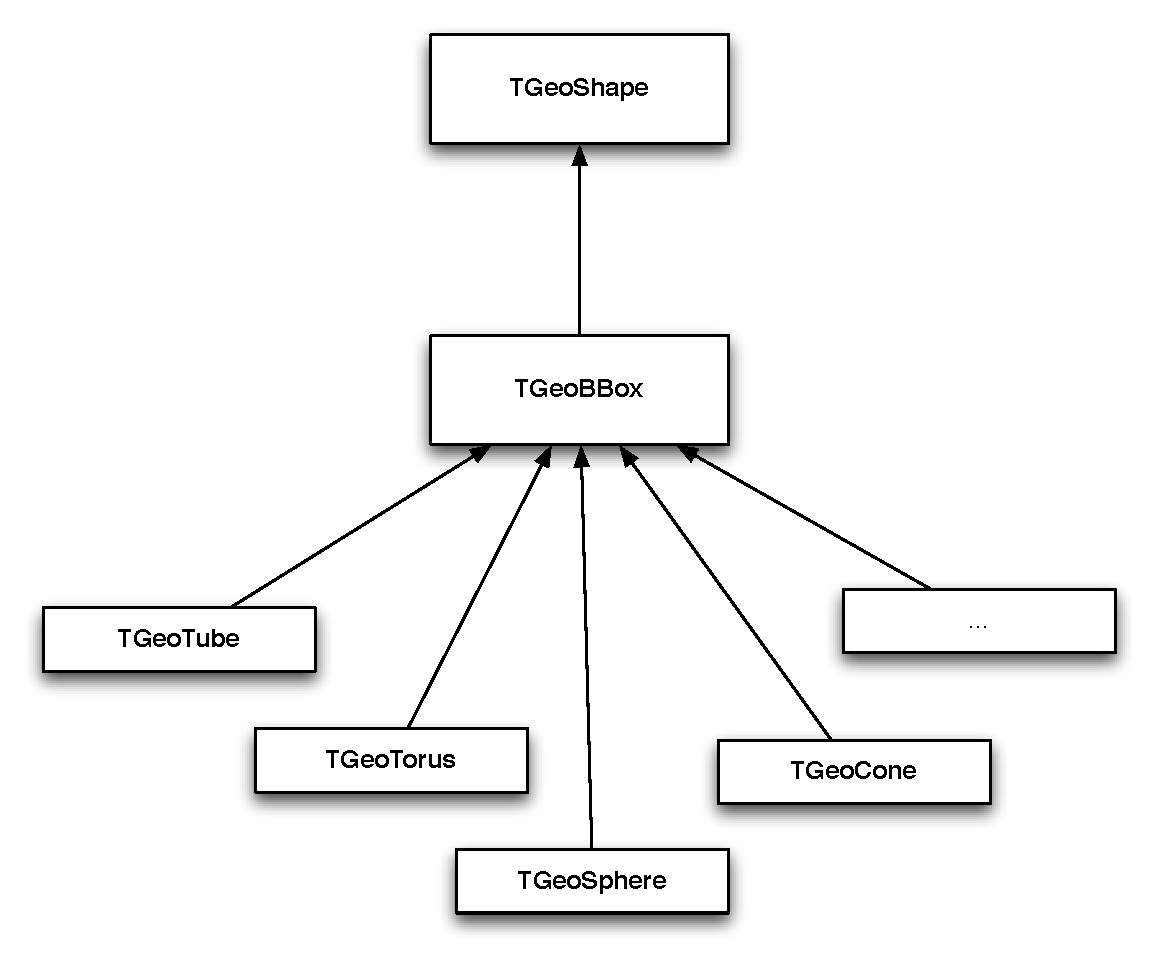
\includegraphics[scale=0.5]{designdocumentimages/ShapeInheritance}
\end{center}
\caption{Graphic depicting the inheritance tree of TGeoShape}
\label{fig:ShapeInheritance}
\end{figure}

From the point of view of track navigation, the most important methods in the shape classes are the two methods to find the distance from a point to the nearest boundary of the shape, in the two cases of the point starting outside the shape, or the point starting from inside the shape. Their interfaces are given in listing~\ref{code:DistFromInside/Outside}.

\begin{sourcecode} 
\begin{lstlisting} [label=code:DistFromInside/Outside, caption=The interfaces of the methods DistFromInside/Outside from TGeoShape.]
Double_t *TGeoShape::DistFromInside(Double_t *point, Double_t *dir, Int_t iact=1, 
                      Double_t step=TGeoShape::Big(), Double_t *safe=0) const = 0;


Double_t *TGeoShape::DistFromInside(Double_t *point, Double_t *dir, Int_t iact=1, 
                      Double_t step=TGeoShape::Big(), Double_t *safe=0) const = 0;

\end{lstlisting} 
\end{sourcecode}

Both methods take a point and a direction in the local coordinate of proper volume they are within as well as a stepsize, and return the distance to the nearest boundary, or if it doesn't find a boundary, returns a very big number to signify that no boundary was reached. This distance is then used by the class TGeoNavigator which is responsible for actually taking a track object and making a step along its trajectory. 

The actual method interface that a programmer using ROOT will interact with to perform basic tracking is not that of the shapes and volumes, but of TGeoManager and TGeoNavigator. The navigator holds several variables describing the current navigation state such as the current position of the track, the current direction of the track, pointers to the current node and the next node that will be reached, as well as numerous flags related to volume boundary conditions such as whether we are sitting on the boundary or approaching from within.

The combined task of finding the distance to the next boundary, and then propagating the current point in this direction to the boundary is handled by the central method to tracking in ROOT, `FindNextBoundaryAndStep'. The interface of this method given in listing~\ref{code:FindNextBoundaryAndStep}. 

\begin{sourcecode} 
\begin{lstlisting} [label=code:FindNextBoundaryAndStep,caption=The interface of FindNextBoundaryAndStep in TGeoNavigator.]
TGeoNode *TGeoNavigator::FindNextBoundaryAndStep(Double_t stepmax, Bool_t compsafe)
{
	// Compute distance to next boundary within STEPMAX. If no boundary is found,
	// propagate current point along current direction with fStep=STEPMAX. Otherwise
	// propagate with fStep=SNEXT (distance to boundary) and locate/return the next 
	// node.
	...
}
\end{lstlisting} 
\end{sourcecode}

The method takes as parameters a maximum distance to propagate the point, and a flag to indicate whether to compute the `safe' distance from the current point (find the distance to the closest boundary in any direction). In order to find the distance to the next boundary, FindNextBoundaryAndStep gets the current node stored by the navigator, from which it can query the volume for a pointer to the current shape, which can do the calculation. The navigator can also query all the daughter nodes of the current volume to find the distance to those boundaries, and eventually choose the distance to the boundary that is crossed first. Finally this distance is used to make a step along a straight line to this intersection point.  

\section{Designing a Parabolic-Tracking Engine with ROOT}

The previous section gave a basic introduction to ROOT's built-in navigation tools, however the goal of UCNSIM is to extend these features to the case of UCN moving under gravity. From the first section we have seen what is required to calculate the distance to a shape's boundary along a parabola. The issues we need to consider are as follows:

\begin{enumerate}
	\item The above parabolic-boundary intersection calculations find the \textbf{time} to reach the boundary. This time is then used to calculate the distance travelled. Then to propagate the particle we need the time again again to substitute into equation~\ref{eqn:GravitationalMotion} - we cannot use the distance in this case, unlike the moving along a straight line. So the time, rather than the distance to the boundary is the most important quantity in the parabolic case. This is an important distinction because the formula for the arc length of a parabola, equation~\ref{eqn:ArcLength}, is not straight-forward to invert. It is far easier to work with time to the boundary as a basis however this will require a change in the way that the FindNextBoundaryAndStep method works.
	\item The elements needed by the parabolic intersection calculation are the current position, the current velocity and the field. Therefore whatever new methods are written to calculate this need an interface which is quite different to that used by ROOT currently. 
\end{enumerate}

It is also a clear design goal of UCNSIM that our program runs independently of the ROOT installation used - i.e: nothing \textit{within} ROOT will be changed, the installation will remain as before. All the changes to be made must happen within the UCNSIM program. This is clearly a desirable goal as the program will then be more portable and easier to keep up-to-date with the latest ROOT installation. However it also introduces a number of challenges in how to implement all of the above, while still retaining the useful navigational features of ROOT discussed in the previous section. We wish to retain as much of ROOT's navigational methods as possible since it is a complex process to track particles through geometries and we do not want to have to reinvent everything from scratch here. 

\subsection{Altering the Shape Hierarchy in UCNSIM}

It is relatively straight forward for a programmer to create their own classes and then compile them into a library to be used when running ROOT. However there are many times when we may wish to extend one of ROOT's classes to include some additional functionality. The C++ way to handle this situation is through inheritance, particularly as we want to keep as much of the ROOT class' interface as possible. However inheritance is a complicated issue in C++ and many of ROOT's classes have been designed with the expectation that no-one will ever inherit from them.

For example, lets consider TGeoShape in ROOT. We mentioned before that TGeoShape defines an interface for every volume to implement the methods to find the distance to a boundary from inside or outside that volume. For parabolic-tracking we would like to have two new methods inside TGeoShape that calculate the time to a boundary along a parabola from inside and outside that volume. These two new methods would then be implemented by each of the shapes in the inheritance tree depicted in figure ~\ref{fig:ShapeInheritance}. How can we do this with inheritance in C++?

Suppose we create a new class - TUCNShape - that inherits publicly from TGeoShape. TUCNShape would inherit all of TGeoShape's methods, but we could then add the two new methods to calculate the time along a parabola. However we would then have to create a new class for all of the shapes where we would implement these two new methods for example TUCNBBox and TUCNTube to name a couple. The inheritance hierarchy would then look as in figure~\ref{fig:UCNMultipleInheritance}.

\begin{figure}[!htbp] 
\begin{center}
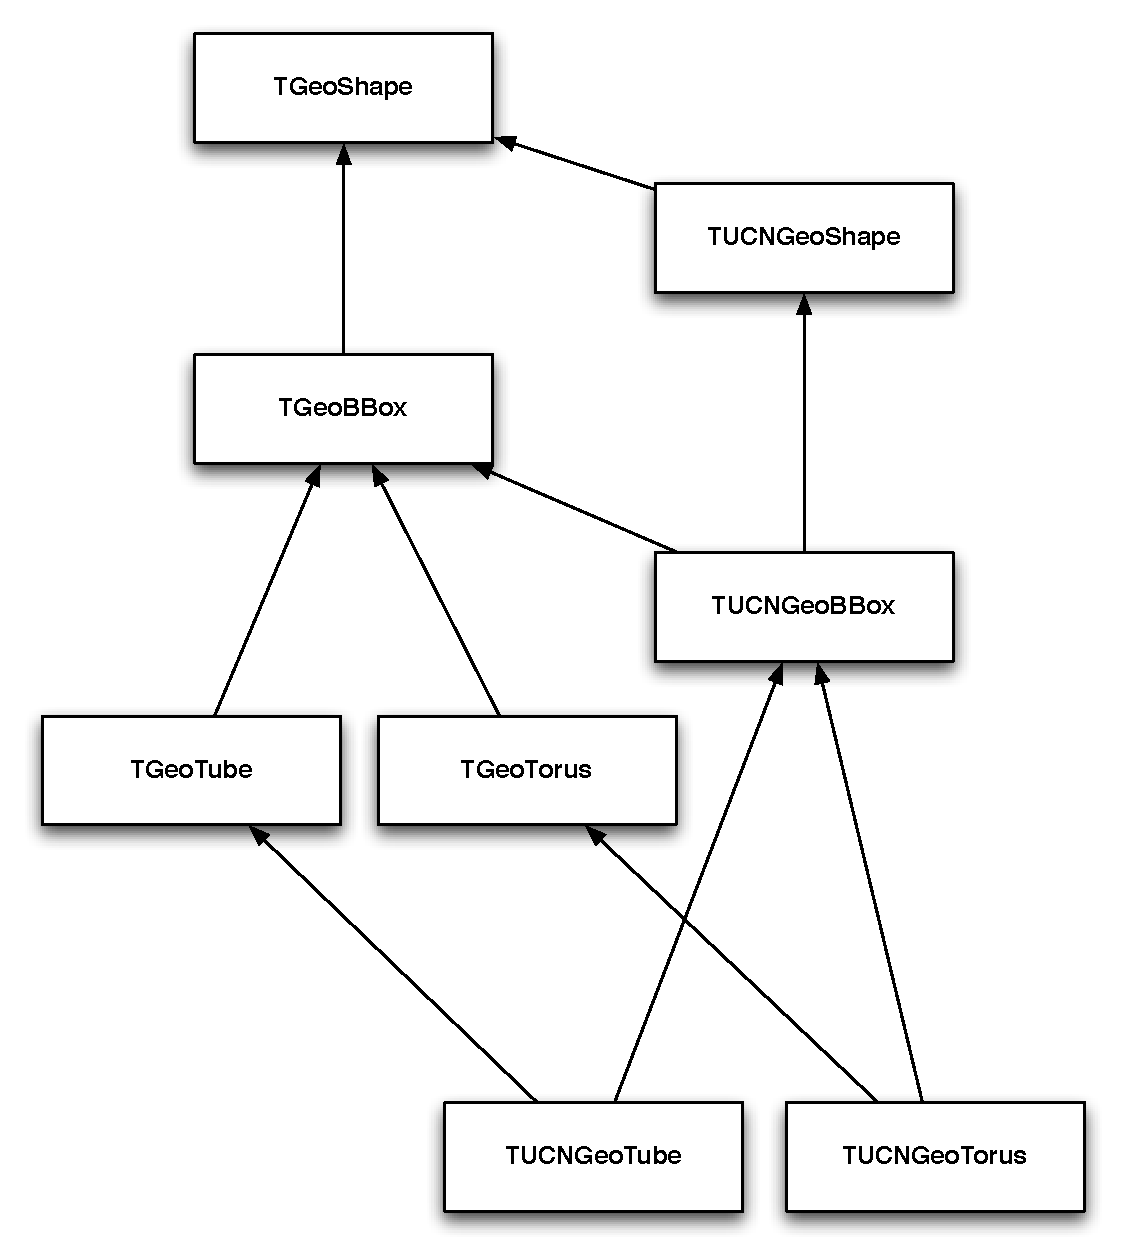
\includegraphics[scale=0.5]{designdocumentimages/MultipleInheritance}
\end{center}
\caption{Graphic depicting the multiple-inheritance problem when trying to make a new class that inherits from TGeoShape}
\label{fig:UCNMultipleInheritance}
\end{figure}

This is a nightmare of multiple-inheritance and even if it could be made to work, would be horrendously fragile and would likely break the polymorphism. To avoid multiple inheritance however, means we have to make a new branch on the shape inheritance hierarchy that defines a new interface in TUCNShape which is then implemenet by TUCNBBox and the `UCN'-shapes, completely bypassing TGeoBBox and the `Geo'-shapes as depicted in figure~\ref{fig:UCNMultipleInheritance2}.

\begin{figure}[!htbp] 
\begin{center}
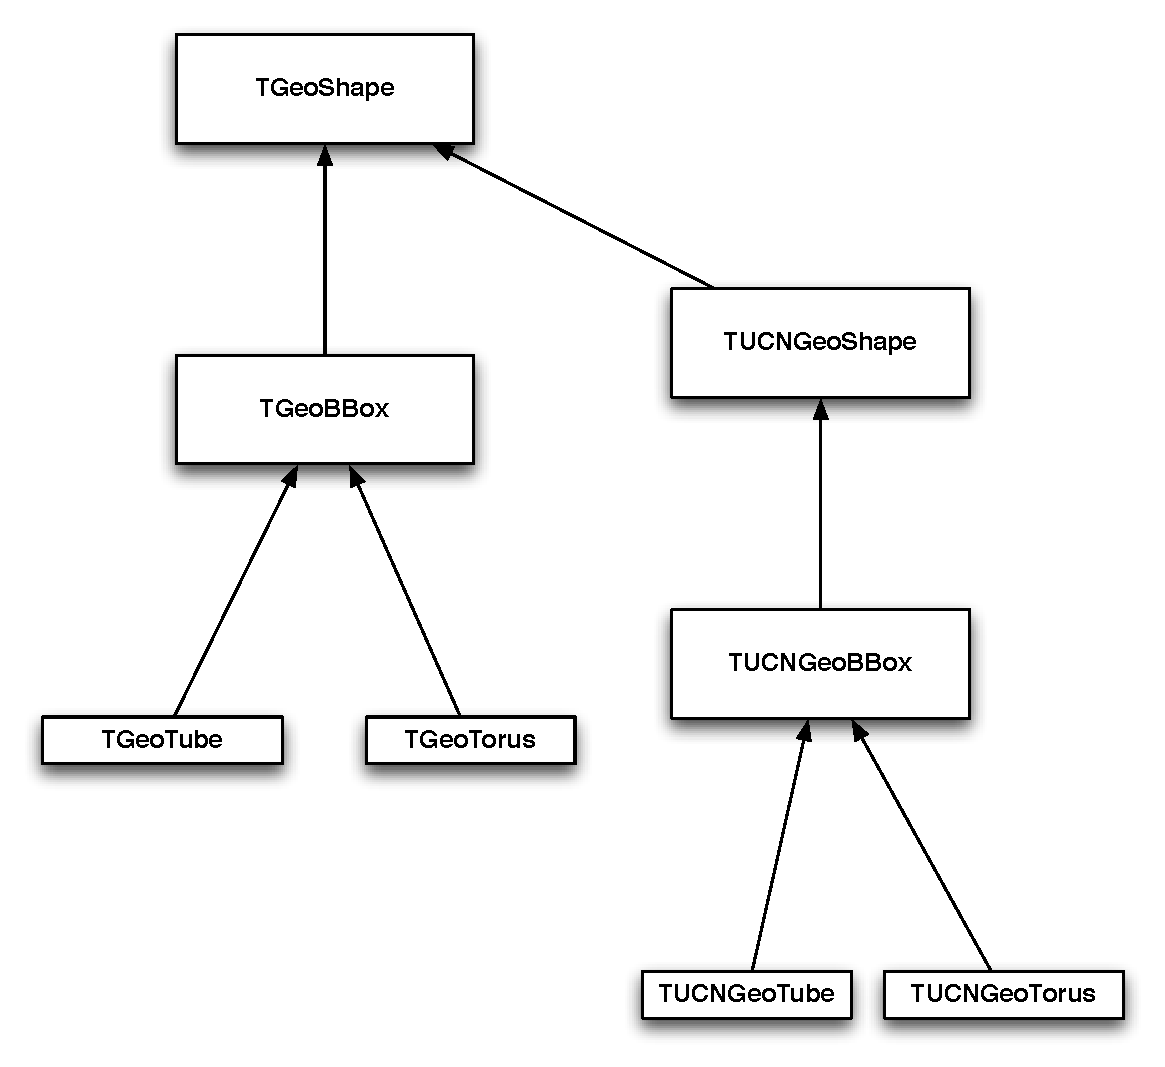
\includegraphics[scale=0.5]{designdocumentimages/MultipleInheritance2}
\end{center}
\caption{Graphic depicting making a sub-inheritance hierarchy that breaks off from TGeoShape}
\label{fig:UCNMultipleInheritance2}
\end{figure}

This approach, however, has two major flaws. The first is that the majority of the new shape classes do not actually inherit from their ROOT counterparts. TUCNBBox is a seperate class from TGeoBBox, despite the fact that we want them to do the same thing except in one specific case. To achieve this then we would have to copy all of the code out of TGeoBBox into TUCNBBox, so the new shape would have all of the same functionality, and then add in our new methods according to the interface laid down in TUCNShape. This is not a very pleasent thing to do, as all of this code is now effectively native to UCNSIM and must be maintained when there are future updates of ROOT. However it would solve the multiple-inheritance problem. 

However the fatal flaw for a scheme like this is that within ROOT itself there are explicit downcasts from a TGeoShape object to a TGeoBBox object. This is possible because in figure~\ref{fig:UCNMultipleInheritance} we see that every object inherits from TGeoBBox - the extra B in TGeoBBox is for `bounding' box, and every other shape type has a corresponding bounding box that perfectly contains the shape. These downcasts would break this system as we would be holding a pointer of type TGeoShape, that points to an object of type TUCNTube say, and would be trying to cast down to pointer of type TGeoBBox which is no longer related to TUCNTube - which would throw an error or crash the program. 

Thus the only solution that preserves the polymorphism, yet lets us alter the class interface is to take the above inheritance tree and move it down a step as in figure~\ref{fig:UCNShapeInheritance}. 

\begin{figure}[!htbp] 
\begin{center}
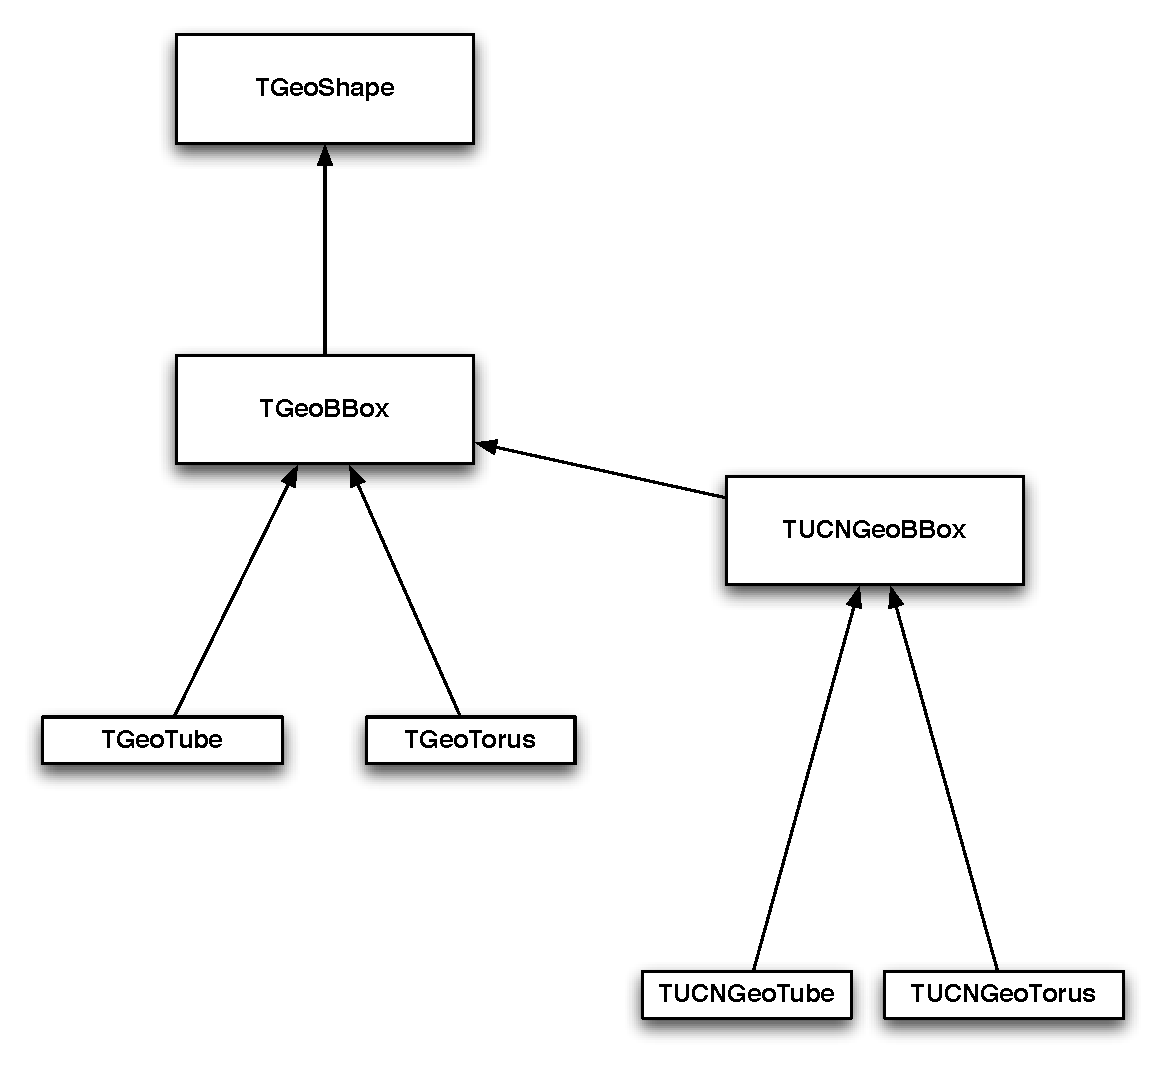
\includegraphics[scale=0.5]{designdocumentimages/UCNShapeInheritance}
\end{center}
\caption{Graphic depicting the final solution of making a sub-inheritance hierarchy that begins at TGeoBBox}
\label{fig:UCNShapeInheritance}
\end{figure}

This scheme still means that we have to copy and paste a lot of code out of ROOT's shapes into UCN-classes, which is most undesirable, however it does mean we have a working inheritance tree that allows us to extend the shapes' interface. Thus we define a new method into TUCNBBox, and implement it for all of the shape classes that we require. Currently these methods have an interface as follows: 

\begin{sourcecode} 
\begin{lstlisting} [label=code:TimeToBoundaryAlongParabola, caption=The interface of the new parabolic-boundary-intersection methods in TUCNGeoBBox.]
Double_t   TimeFromInsideAlongParabola(Double_t* point, Double_t* velocity, 
							Double_t* field, Double_t stepmax=TGeoShape::Big(), 
							Int_t iact=1, Double_t *safe=0) const;
Double_t   TimeFromOutsideAlongParabola(Double_t* point, Double_t* velocity,
	 						Double_t* field, Double_t stepmax=TGeoShape::Big(),
	 						Int_t iact=1, Double_t *safe=0) const;
\end{lstlisting} 
\end{sourcecode}

Another consequence of effectively creating a new inheritance tree of shapes starting from TGeoBBox is that, given a pointer to our new shape class, which is of type TGeoShape (which is how all pointers to shapes are stored in the GeoManager), we must now introduce more casts into the program to cast-down to TUCNGeoBBox, so that we can access the new methods. Casting down is unsafe, unless you can guarantee that the object handed to you is of type TUCNGeoBBox or inherits from it. If it doesn't, then the program will crash. Thus we introduce another requirement to the program by doing this: \textbf{every} shape must be of type TUCNGeoBBox or of a type that inherits from this. 

\subsection{Altering the Navigator in UCNSIM}

The other major change to ROOT's tracking methods that we need to make is in TGeoNavigator. The method FindNextBoundaryAndStep needs to be either replaced by something that takes into account gravitational tracking, or we need a new method to do this. The choice is made for us by the fact that all of the methods in TGeoNavigator are not `virtual', that is, by making a class TUCNGeoNavigator that publicly inherits from TGeoNavigator, we cannot alter the implementation of any of its methods. Therefore we have to introduce more new methods to our program. However new methods mean more explcit casting down from a pointer to the base object. In this case we don't have any other option since our hands are tied by the design of the TGeoNavigator class - it was never designed to be inherited from. 

The class TUCNGeoNavigator then implements a new method, 

\begin{sourcecode} 
\begin{lstlisting} [label=code:FinNextBoundaryAndStepAlongParabola, caption=The interface of FindNextBoundaryAndStepAlongParabola]
TGeoNode*	FindNextBoundaryAndStepAlongParabola(TVirtualGeoTrack* track, 
						TUCNGravField* field, Double_t stepTime, Bool_t compsafe=kFALSE);
\end{lstlisting} 
\end{sourcecode}

FindNextBoundaryAndStepAlongParabola follows the algorithms used by FindNextBoundaryAndStep closely, as this is a very large and complicated function that checks numerous volumes and flags to ensure that the point is propagated to the correct place and that the relevant information is updated correctly. Where it differs is in how it propagates the point (along a parabola) and how it finds the distance to the boundary. As mentioned above, we work predominantly with the time to intersect the boundary, which we get by taking the pointer to the current shape and casting down to type TUCNGeoBBox, to allow us to call the new methods to calculate the time to intersect the boundary. Beyond this, the rest of the function's logic is kept as close as possible to the original except where this is not possible. 

One place where we have to make more changes are the flags to indicate the state of the particle with respect to the boundary. These flags are private data members with accessor methods, but no mutator methods to change their value. They are hardcoded into TGeoNavigator's methods and always changed explicitly. This is a problem as an inherited class cannot access the base class' private data members, and so, if we cannot update these state flags, they are useless to us. To get around this problem, the only thing we can do is create new flags in TUCNGeoNavigator that exactly replicate the function of the old flags. This is another ugly compromise as you then have an object holding two sets of flags, one of which contains information and the other set which is uninitialised or worse. 

Other methods in TGeoNavigator check these flags and implement them in their logic, so this may not only be ugly, but also detrimental to the proper functioning of the program. The only way to solve this problem though is to once again, copy all of the TGeoNavigator code into the new class and break the inheritance relationship, using TUCNGeoNavigator exclusively. This is perhaps an even uglier solution, as the TGeoManager must then also be modified to only use the TUCNGeoNavigator class rather than the TGeoNavigator class, which means more code must be copied into UCNSIM and changed. 

There are no other options to resolve this problem at present short of asking the developers of ROOT to make all of the class virtual in these classes, and include mutator methods for all of the private data members. 

\subsection{Overview of UCNSIM Class Structure}

Having discussed some of the major design issues and compromises that had to be made to create a sub-library of classes that utilise ROOT's navigational features, yet extend them to include gravitational tracking, we are now in a position to look at the current class structure of UCNSIM. Hopefully it will now be clear why certain classes inherit from ROOT and others are standalone classes. Remember that every inheritance relationship means more explicit casts in the program, so we want to keep inheritance to a mimimum. 

\begin{figure}[!htbp] 
\begin{center}
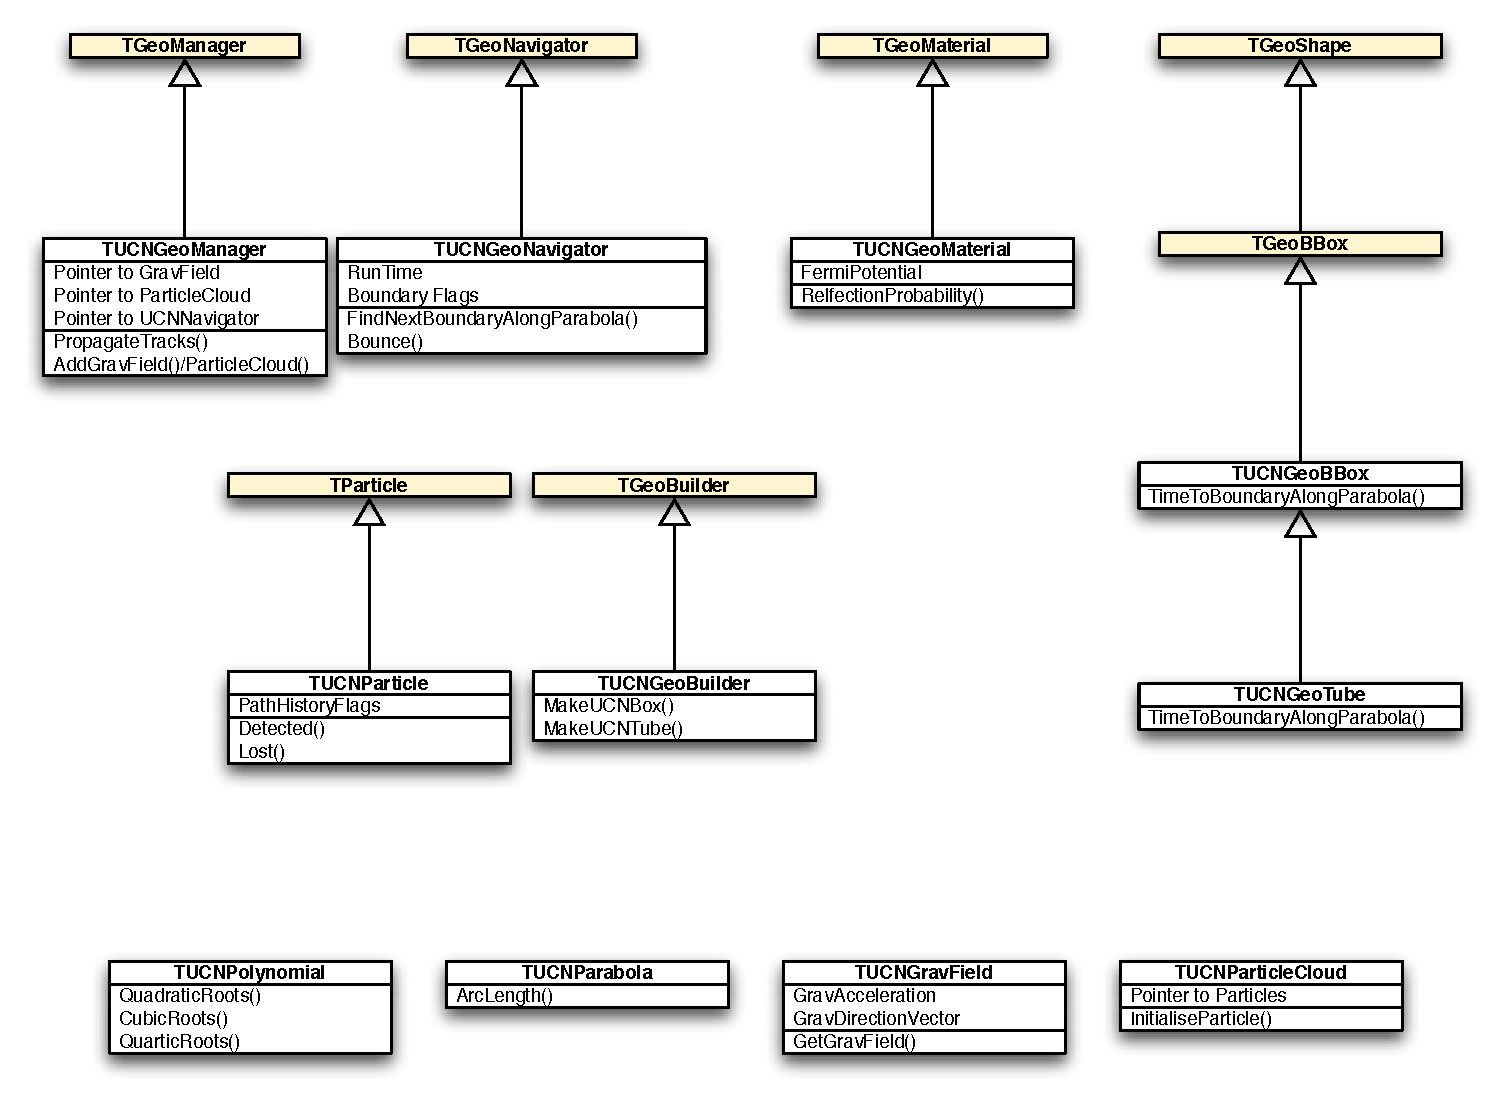
\includegraphics[scale=0.7]{designdocumentimages/UCNSIMClassStructure}
\end{center}
\caption{Class diagram for the UCNSIM program}
\label{fig:UCNSIMClassStructure}
\end{figure}

We have already discussed the shape and navigator classes in relative detail. Other inherited classes include the TUCNGeoManager and TUCNGeoBuilder, which both add new methods to create volumes from the TUCNGeoShapes we must now create to get gravitational tracking. TUCNGeoManager holds pointers to new classes such as the TUCNParticleCloud which creates and holds the list of particles, as well as the class TUCNGravField. The final inherited class is the TUCNParticle, which only adds a few new methods to make accessing certain data relevant to UCN simpler as well as holding flags as to the final status of a particle, for example, was it lost or detected or still propagating. The classes TUCNPolynomial and TUCNParabola are singletons holding root-finding algorithms or the methods to calculate much needed quantities. TUCNMaterial holds physical quantities such as the fermi potential, relevant to the behaviour of the neutrons at the boundary.

Ultimately the package of classes tie together closely, so any program in UCNSIM must use these objects exclusively in place of their base classes. 


\section{Summary}

In conclusion, the design of UCNSIM is severely hampered by the need to introduce new functionality into ROOT's classes without actually changing the ROOT installation at all. Inheriting from classes that were not designed to be inherited from is a gauntlet that only gets harder to traverse. However, in spite of this, there are ways to build a program with the required functionality that although lacking elegance and simplicity, do work when conditions are followed as to the set-up of the program. 

\subsection{Planned Features and Future Timetable}

UCNSIM in its current state supports particle gravitational particle tracking in two volumes - the Box and the tube. The behavior of UCN interacting with a boundary have also been implemented, with support for absorption/inelastic scattering at the boundary as well as specular/non-specular reflection at a boundary according to a fixed probability. 

\textbf{Longer Term Plan and Intended Upcoming Features:} \\

\begin{center}
    \begin{tabular}{ | p{3cm} | p{8cm} | l |}
    \hline
    Feature & Description & Timeline \\ \hline
    Magnetic Field Environment & To build an interface to incorporate magnetic fields, either defined by a function or by a field map. & October 2009 \\ \hline
    Spin Vector Tracking & Introduce a spin vector to the particles with algorithms to simulate the dynamics under the magnetic field environment & December 2009 \\ \hline
	 Multiple Volume Environments & Test program's scalability with larger and larger arrays of interconnected volumes, making improvements where necessary & Janurary 2009 \\ \hline
	 Collect Present Experimental Data & Collect as much data from the collaboration as possible relating to previous runs with neutrons. Try to test simulation against whatever data can be found & February 2009 \\ \hline
	 ROOT Geometry of the experiment & Create and test simulations of a full experimental mockup, checking filling times and tracking of neutrons throughout the whole system & March 2009 \\ \hline
	 EDM Data and Analysis & Develop a system incorporating a neutron EDM as a simulation parameter and try to extract this value from simulated spin precession frequency data. & May 2009 \\ \hline
    \end{tabular}
\end{center}




\end{document}
